%% W3 (#134). Budget 2.3pp. THE CENTREPIECE.
%%
%% DO NOT RECOMPUTE ANYTHING. Every number already exists:
%%   tmp/b1_sham_control.md          sham control, 2000 exact-matched partitions
%%   tmp/b2_ehr_only.md              features predict survival, AUROC + CIs
%%   tmp/c1_temporal_cutoff.md       coverage table, base-rate collapse
%%   tmp/c117_fixed_window.md        G2 recall 0.8163 -> 0.3048 under 24h
%%   tmp/a5_headline_numbers.md      pooled clean-split numbers, floor failures
%%   tmp/b6_intervals.md             fragility of all 56 cells
%%   tmp/t4_24h_sham_precheck.md     fresh 24h run, no usable partition
%%   tmp/t5_discovery.md             (if T5 #128 lands in time; optional)
%%
%% Requirements from W1:
%%   - ONE summary table carrying each control, what it tests, its result. A
%%     reviewer should be able to read that table alone and get the paper.
%%   - Every number annotated with the tmp/ report it came from, in a comment.
%%   - CIs on every proportion (B6). No bare point estimates.
%%   - State the honest asymmetries rather than burying them: the 5x gain at
%%     P>=0.98 narrows to 1.34x at P>=0.95; the 0.98 precision figure rests on
%%     3 false positives; percentiles are not comparable across partition shapes.
\section{Results: What Each Control Found}
\label{sec:results}
\todo[inline]{W3 (\#134): draft.}

%% --- Carried over from ictai2026, kept per W1 S4. RELABEL: this is the result
%% --- being examined, not a result. Caption must say in-sample.
\begin{figure}[t]
    \centering
    % Recall versus minimum-precision floor for each trimmed-tree sub-group.
% Data is the same as Table~\ref{tab:fdp_recall_nosurv} (target class = Non-survivor)
% produced by filter-repository-python/compute_fdp_and_recall.py. The
% precision floor decreases left-to-right so the curve sweeps from the
% strict strong-filter regime (P = 1.00) to a relaxed P >= 0.95 cut.
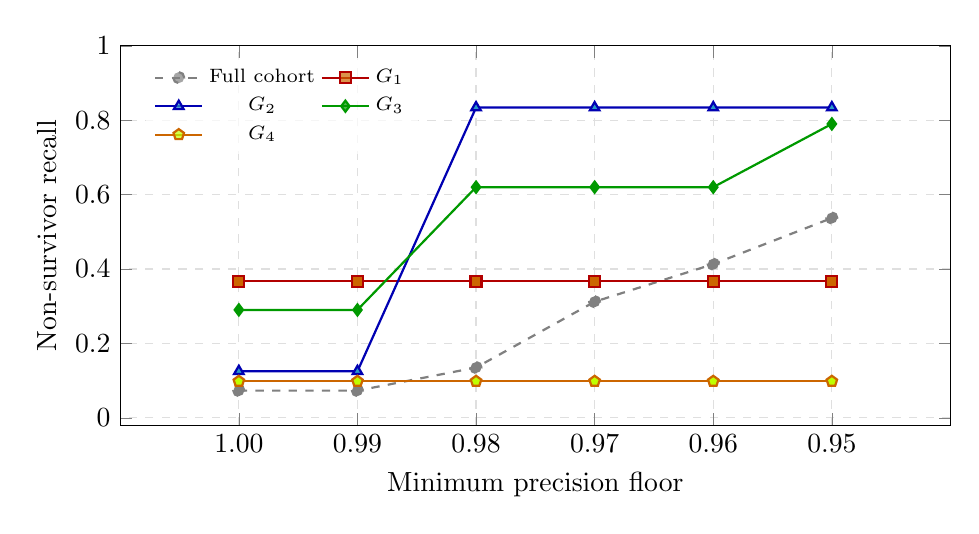
\begin{tikzpicture}
    \begin{axis}[
        width=\linewidth,
        height=6.4cm,
        xlabel={Minimum precision floor},
        ylabel={Non-survivor recall},
        xmin=0.94, xmax=1.01,
        ymin=-0.02, ymax=1.0,
        x dir=reverse,                 % strict (P=1) on the left
        xtick={1.00, 0.99, 0.98, 0.97, 0.96, 0.95},
        xticklabel style={
            /pgf/number format/.cd, fixed, fixed zerofill, precision=2,
        },
        ytick={0, 0.2, 0.4, 0.6, 0.8, 1.0},
        grid=major,
        grid style={dashed, gray!25},
        legend style={
            at={(0.03, 0.97)},
            anchor=north west,
            draw=none,
            fill=white,
            fill opacity=0.7,
            text opacity=1,
            font=\scriptsize,
            legend columns=2,
        },
        cycle list name=exotic,
    ]

    % ---- Full cohort (dashed, gray); n=658, matches Table~\ref{tab:fdp_recall_nosurv} ----
    \addplot+[mark=*, thick, dashed, gray, mark options={fill=gray}]
        coordinates {
            (1.00, 0.073) (0.99, 0.073) (0.98, 0.135)
            (0.97, 0.312) (0.96, 0.413) (0.95, 0.537)
        };
    \addlegendentry{Full cohort}

    % ---- G1 ----
    \addplot+[mark=square*, thick, red!70!black]
        coordinates {
            (1.00, 0.367) (0.99, 0.367) (0.98, 0.367)
            (0.97, 0.367) (0.96, 0.367) (0.95, 0.367)
        };
    \addlegendentry{$G_1$}

    % ---- G2 ----
    \addplot+[mark=triangle*, thick, blue!70!black]
        coordinates {
            (1.00, 0.125) (0.99, 0.125) (0.98, 0.834)
            (0.97, 0.834) (0.96, 0.834) (0.95, 0.834)
        };
    \addlegendentry{$G_2$}

    % ---- G3 ----
    \addplot+[mark=diamond*, thick, green!60!black]
        coordinates {
            (1.00, 0.290) (0.99, 0.290) (0.98, 0.620)
            (0.97, 0.620) (0.96, 0.620) (0.95, 0.790)
        };
    \addlegendentry{$G_3$}

    % ---- G4 (merged Stable / ambiguous) ----
    \addplot+[mark=pentagon*, thick, orange!80!black]
        coordinates {
            (1.00, 0.098) (0.99, 0.098) (0.98, 0.098)
            (0.97, 0.098) (0.96, 0.098) (0.95, 0.098)
        };
    \addlegendentry{$G_4$}

    \end{axis}
\end{tikzpicture}

    \caption{Non-survivor recall against the precision floor, full cohort and
    each subgroup. \todo[inline]{W3 (\#134): rewrite caption --- must state that
    thresholds here are selected \emph{in-sample}, and that this is the result
    the controls go on to examine.}}
    \label{fig:recall_vs_precision}
\end{figure}

%% Citation smoke test -- verifies ACM-Reference-Format resolves. W3 may remove.
The pipeline under examination is described in~\cite{bradland_knowledge-informed_2025}
and its downstream filter in~\cite{zadorozhny_towards_nodate}.
